\documentclass[12pt, twocolumn]{article}
% \documentclass[12pt]{article}
\usepackage[margin=2.5cm]{geometry}
\usepackage{enumerate, fancyhdr, graphicx, amsmath, lipsum, wrapfig, nameref, url, hyperref}

\title{Ideal Climb Angle for Mars Rovers}
\author{Paul Chesnais (pmc85)}
\date{\today}

\pagestyle{fancy}
\fancyhead{}
\lhead{Paul Chesnais (pmc85)}
\chead{ASTRO 3310 - HW\#1}
\rhead{\today}
\fancyfoot{}
\rfoot{\thepage}
\lfoot{
\includegraphics[height=20pt]{Logo}}
\renewcommand{\headrulewidth}{0.5pt}
\renewcommand{\footrulewidth}{0.5pt}

\usepackage[binary-units=true]{siunitx}
\sisetup{load-configurations = abbreviations}

\newcommand{\e}{&=}
\newcommand{\p}[1]{\times 10^{#1}}

\begin{document}
\maketitle
\thispagestyle{empty}

\section{Abstract}
\label{sec:abstract}
Exploring Mars, or any planet for that matter, isn't easy. Especially since as of right now, rovers are the only things capable of doing it. Unfortunately, designing rovers is incredibly difficult. Given the topology for a particular landing site, how do you optimize each component of a rover? Suppose the craft were fitted with a more powerful engine to clear large humps. This would make the rover heavier, and therefore harder to land. Designing such crafts is full of conundrums. This project hopes to help in making such critical decisions. Given topographical data on candidate landing sites on Mars, how does the maximum climb angle affect the total explorable distance?

\begin{figure*}
  \includegraphics[width=\textwidth]{figures/Mars_relief.png}
  \caption{Colorized Mars Relief}
  \label{fig:mola}
\end{figure*}

\section{Datasets}
\label{sec:datasets}
\par NASA and ESA have been working very hard to map out Mars' topography. Figure~\ref{fig:mola} shows us relief of Mars captured by the Mars Orbiter Laser Altimeter (MOLA) from the Mars Global Surveyor mission \cite{bib:mola}that ran from 1997 to 2006. This particular dataset has an accuracy of about \SI{460}\m{} per pixel \cite{bib:nasa-review}. Unfortunately, as accurate as this data is, it is not accurate enough. Though the average slope over those \SI{460}\m{} may be climbable by a certain rover, there may be some irregularities that the rover cannot climb.
\par Fortunately, the ESA has sent a mission more recently than NASA called Mars Express, on board which a camera called High/Super Resolution Stereo Colour Imager (HSRC) \cite{bib:hsrc}. This particular camera captures images with an accuracy of \SI{10}\m{} per pixel, meaning that the datasets are very very accurate and better suited for our purposes. They have been collecting data around Mars for close to 12 years now, and while data is still being received, a lot of Mars' topography has been mapped and refined since, at very very high accuracy.
\begin{figure}[h!]
  \center
  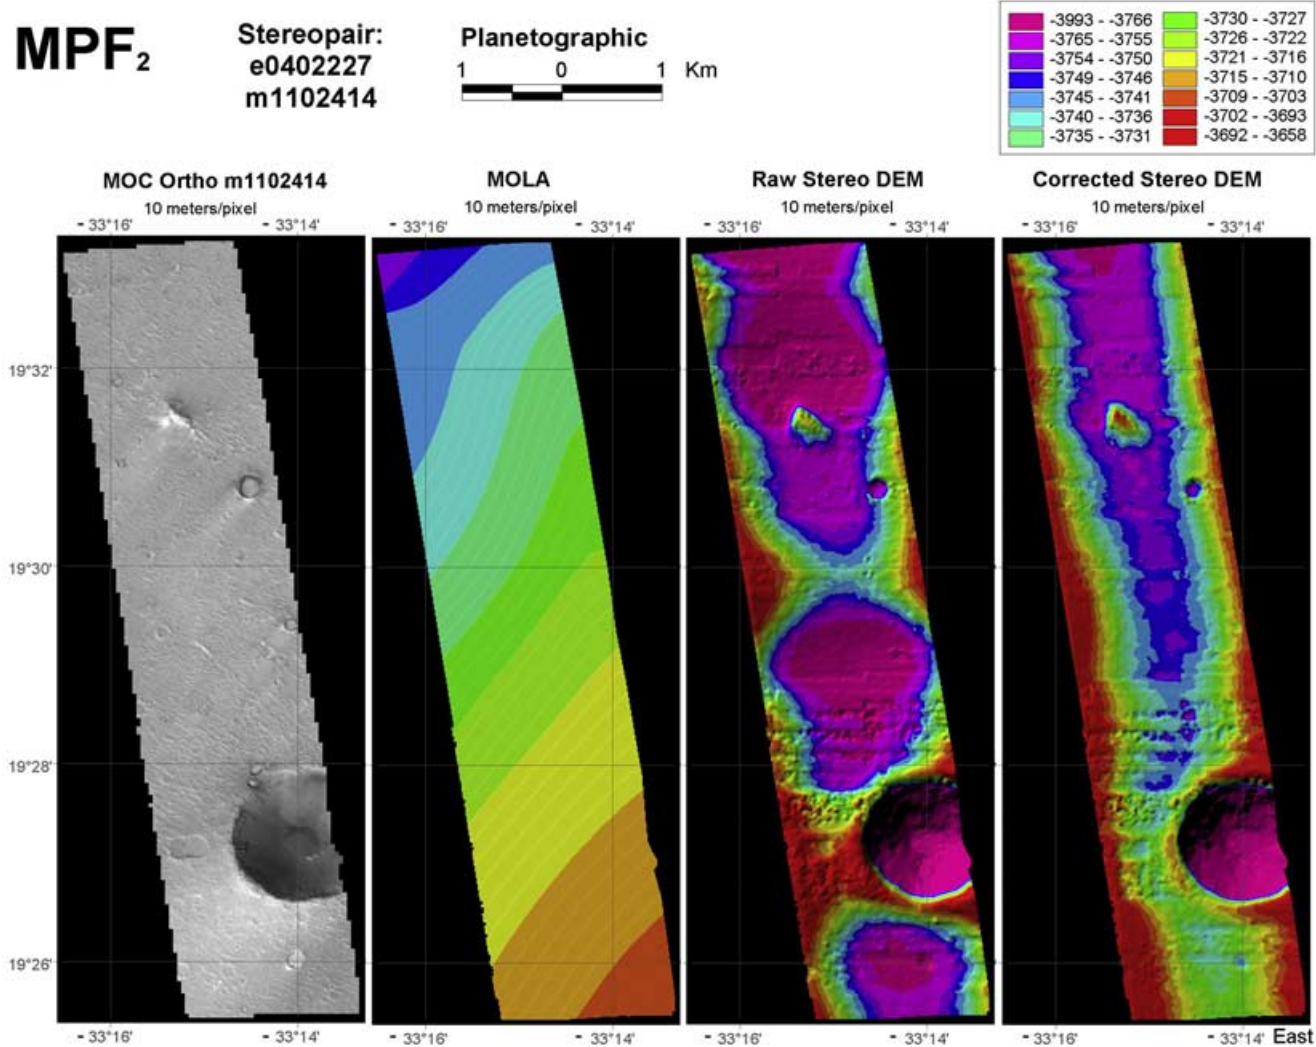
\includegraphics[width=0.5\textwidth]{figures/pathfinder.png}
  \caption{Mars Pathfinder Landing Site Topography}
  \label{fig:pathfinder}
\end{figure}
\par Others have been working very hard to map out topographical data for possible landing sites. The U.S. Geological Survey's Astrogeology Team \cite{bib:landingsites} has studied Mars Orbiter images to produce elevation models. Using multiple techniques, such as photoclinometry, they were able to produce topography maps at extremely high resolutions, up to \SI{3}\m{} per pixel. Figure~\ref{fig:pathfinder} shows the calculated topography of the Mars Pathfinder landing site. In this Figure, the technique used was stereo photogrammetry. They achieved a \SI{10}\m{} per pixel accuracy, which is far more accurate and more in the range of data required for this project.


% \begin{figure}
% 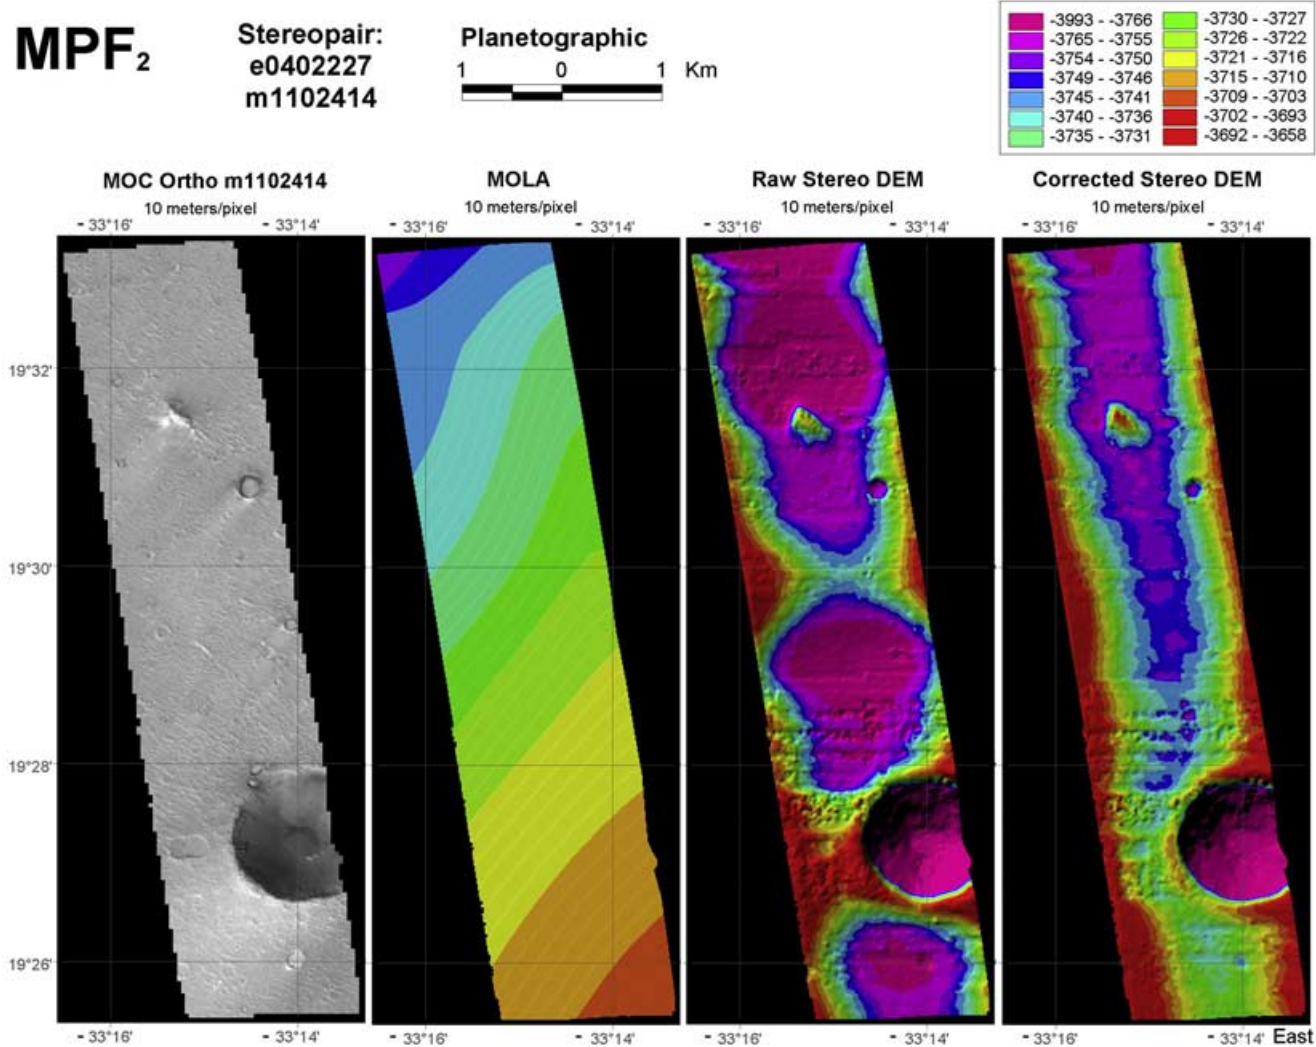
\includegraphics[height=10cm]{figures/pathfinder.png}
% \caption{Gusev Crater Image Resolution}
% \label{fig:gusnev}
% \end{figure}

\section{Methods}
\label{sec:methods}
\par Often mentioned in the \nameref{sec:datasets} section is accuracy, especially one unit of accuracy: meters per pixel. This unit is important because it effectively represents the distance between altimetry data points. If this distance is far too large relative to the size of the rover, then studying this data in the hopes of finding the ideal angle is pointless. On the other hand, with datasets like the ones received from the Mars Express mission, with an accuracy of \SI{10}\m{} per pixel and a rover \SI{3}\m{} long (like Curiosity), meaningful calculations can be made.
\par Once right the datasets are chosen, designing the algorithm can start. First, a 2D array of altimetry data can just as easily be treated as a graph, meaning that graph traversal techniques can be used. Given the potential size of the graph, it would be unwise to traverse it multiple times, once for each angle. Therefore we need to traverse the graph and record the minimum required climb angle to get to every node. Below is a step by step procedure that takes an altimetry graph and a starting position, and outputs a graph where each node is associated with its respective minimum climb angle:
\begin{enumerate}
  \item For each neighbor of the current node, calculate the height difference over the distance.
  \item If the slope to the neighbor is too steep, define its minimum climb angle to be infinite. Else, define it to be the calculated slope. If the neighbor has already been visited, and therefore already has a minimum climb angle associated to it (infinite or otherwise), set it to be the minimum of the current calculated minimum climb angle, and the previously calculated climb angle.
  \item Call this function on each neighbor reachable from the current point.
\end{enumerate}
Finally, go through the graph once more and keep a record of the number of node associated with each minimum climb angle to produce a graph plots minimum climb angle versus nodes reached (i.e. area covered).

\par This algorithm is a slightly modified version of Depth First Search, where the main difference is that it is allowed to revisit nodes if it has found a path to it that requires a smaller climb angle. It is also very practical because it does not require that the whole dataset fit into memory (though it would dreadfully slow if it did not). Graph traversal is also, in theory, parallelizable. But, doing so for this algorithm would also be far beyond the scope of this class, so only the serial version of this algorithm will be implemented.

\section{Conclusions}
\label{sec:conclusions}
A plot that shows a rover's maximum climb angle versus total area coverable would be extremely useful in making decisions when designing a mission. This project hopes to produce such a plot for all candidate landing sites of Mars, and potentially beyond, in order to provide teams with this help.

\begin{thebibliography}{1}
\bibitem{bib:mola}
\url{http://pds-geosciences.wustl.edu/missions/mgs/mola.html}
\bibitem{bib:landingsites}
\url{http://webgis.wr.usgs.gov/pigwad/publications/2003JE002131.pdf}
\bibitem{bib:hsrc}
\url{http://pds-geosciences.wustl.edu/missions/mars_express/hrsc.htm}
\bibitem{bib:nasa-review}
\url{http://www.marsjournal.org/contents/2008/0002/files/som_mars_2008_0002.pdf}
\end{thebibliography}

\end{document}